% begin module trig-functions
\begin{frame}
\frametitle{Trigonometric Functions and Right Angle Triangles}
\vskip -0.05cm
\hfil $
\begin{array}{|cc|cc|}
\hline
\multicolumn{2}{|c|}{%

\psset{xunit=1cm,yunit=1cm}
\begin{pspicture}(-4,-0.5)(1,2.5)
\tiny
\psaxes[labels=none, ticks=none]{<->}(0,0)(-4,-0.5)(1,2.5)
\pscircle*(-3,2){0.07}
\psline(0,0)(-3,2)
\psarc[linecolor=red](0,0){0.5}{0}{146.3099}
\rput[br](-3.1, 2){$(x,y)$}
\rput[l](0.1, 0.7){$\theta$}
\rput[lb](-1.55, 1.1){$r$}
\psline(-3, 2)(-3, 0)
\only<handout:0|3,4,5,7>{\psline[linewidth=2pt, linecolor=blue](-3, 2)(-3, 0)}
\only<handout:0|2,4,5,6>{\psline[linewidth=2pt, linecolor=green](0, 0)(-3, 0)}
\only<handout:0|2,3,6,7>{\psline[linewidth=2pt, linecolor=orange](0, 0)(-3, 2)}
\psline[linestyle=dotted](-3, 2)(0, 2)
\psline[linecolor=red](-2.7, 0)(-2.7, 0.3)(-3, 0.3)
\psline(0, 1.7)(-0.3, 1.7)(-0.3, 2)
\end{pspicture}
%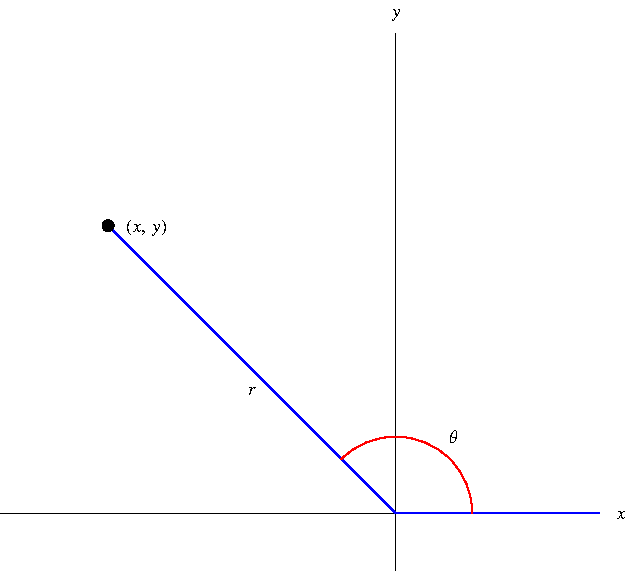
\includegraphics[width=5cm]{trigonometry/pictures/app-d-ratiosb.pdf}%
}&%
\multicolumn{2}{|c|}{%
\psset{xunit=1cm,yunit=1cm}
\begin{pspicture}(0,0)(5,3)
\tiny
\psline(0,0)(4.5,0) (4.5,3)(0,0)
\psline(4.2,0)(4.2, 0.3)(4.5,0.3)
\rput(0.8, 0.3){$\theta$}
\rput(2.7,0.2) {\tiny adjacent}
\rput[b]{90}(4.4,1.5) {\tiny opposite}
\rput{! 2 3 div  ATAN 57.295779513 mul}(2.25,1.7){\tiny hypotenuse}
\psarc[linecolor=red](0,0){0.5}{0}{33.690067526}
\end{pspicture}
%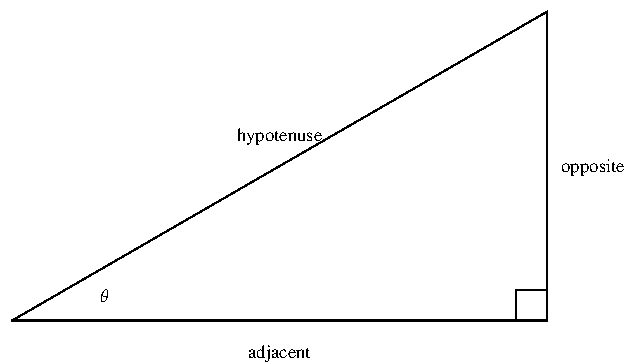
\includegraphics[width=5cm]{trigonometry/pictures/app-d-ratiosa.pdf}%
}%
\\%
\cos \theta \uncover<3->{= \frac{ x}{ r}} &
\sec \theta \uncover<6->{= \frac{ r}{ x}} &
\sin \theta = \frac{\textrm{opp}}{\textrm{hyp}} &
\csc \theta = \frac{\textrm{hyp}}{\textrm{opp}} 
\\
\sin \theta \uncover<2->{=  \frac{\only<handout:0|2>{\color{blue}} y}{\only<handout:0|2>{\color{orange}} r}} 
&
\csc \theta \uncover<7->{= \frac{ r}{ y}} &
\cos \theta \uncover<4->{= \frac{\textrm{adj}}{\textrm{hyp}}} &
\sec \theta \uncover<4->{= \frac{\textrm{hyp}}{\textrm{adj}}}
\\
\tan \theta \uncover<4->{= \frac{ y}{ x}} &
\cot \theta \uncover<5->{= \frac{ x}{ y}} &
\tan \theta \uncover<4->{= \frac{\textrm{opp}}{\textrm{adj}}} &
\cot \theta \uncover<4->{= \frac{\textrm{adj}}{\textrm{opp}}}
\\
\hline
\multicolumn{2}{|c|}{\text{All angles}}&
\multicolumn{2}{|c|}{\text{Acute angles}}
\\
\hline
\end{array}
$

\begin{itemize}
\item The trigonometric functions can be defined without requesting that the pt. $(x,y)$ on the terminal arm of the angle lie on the unit circle.
\item<2-> To do so we rescale by the distance $r$ from the origin.
\item The trig functions of acute $\alpha$ can be interpreted as ratios of sides of right angle triangle with one angle equal to $\alpha$.
\end{itemize}

\end{frame}
% end module trig-functions